\section{Resultater}

Testsignalerne er placeret som vist i nedenstående tabel.

\begin{tabular}{p{3.2cm}|p{2.3cm}|p{2.3cm}|p{2.3cm}}
	Testsignal nr. & Azimuth i grader & Elevation i grader & Distance i meter \\\hline
	Referencesignalet & 0 & 0 & 1 \\
	1 &90&0&1 \\
	2 &270&0&2 \\
	3 &180&0&1 \\
	4 &180&-30&1 \\
	5 &0&30&1 \\
	6 &60&10&3 \\
	7 &240&-10&0.5 \\
	8 &5&-20&1.1 \\
	9 &0&90&2 \\
	10 &135&0&9.8 \\
\end{tabular}

Med alle indsamlede data fra lyttetestene, laves plottet på figur \ref{fig:allplots}. Her ses det, at selvom en del af resultaterne rammer nogenlunde indenfor de angivne testsignaler, er der mange svar som er placeret meget langt fra testsignalerne. 



\begin{figure}
	\centering
	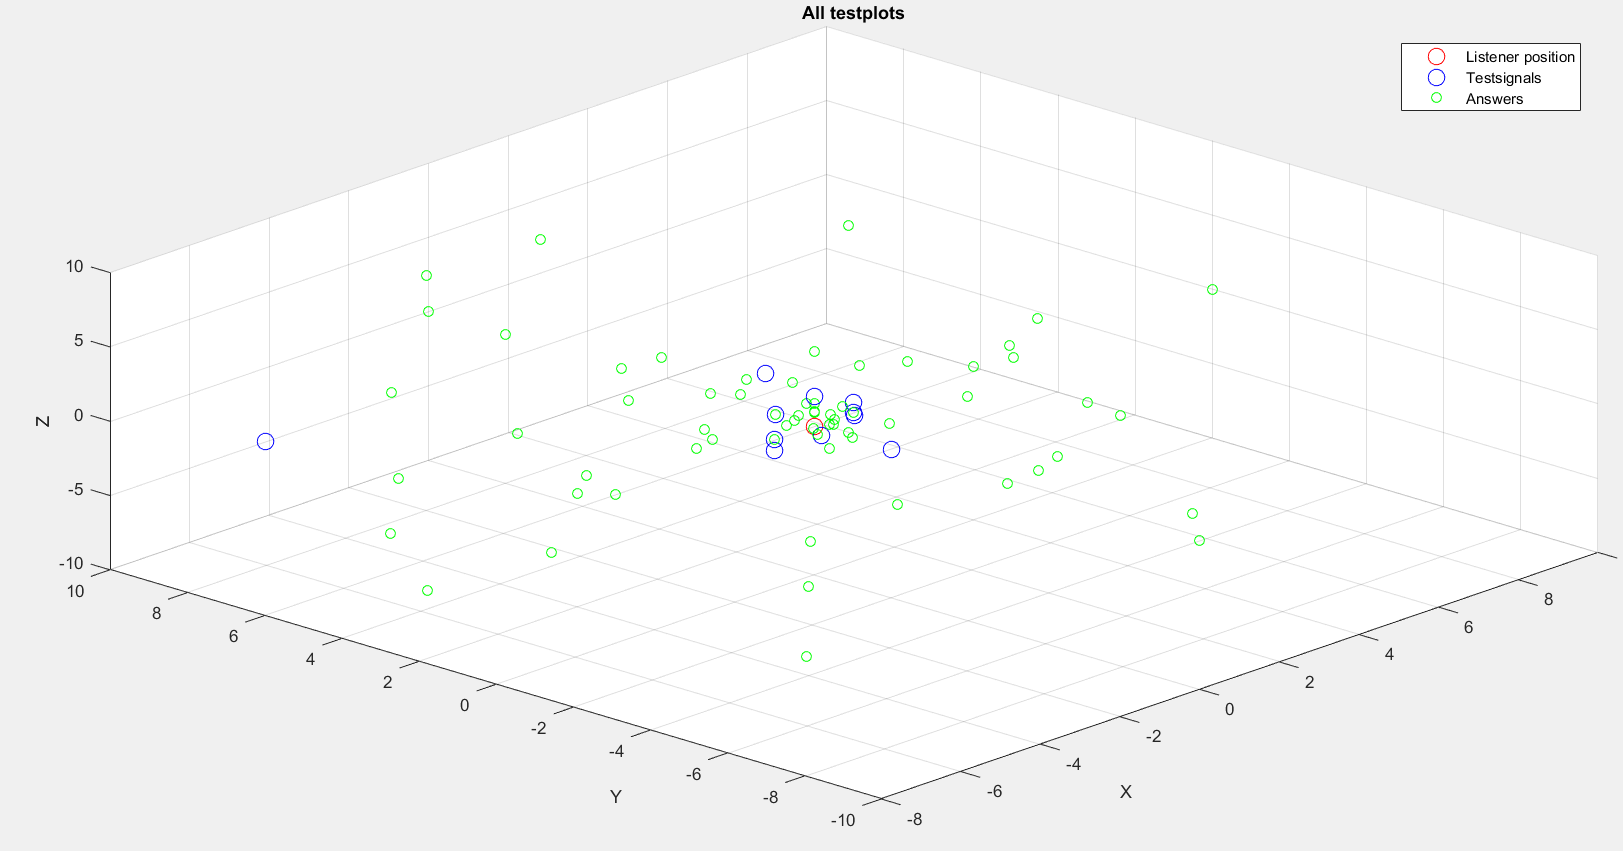
\includegraphics[width=1\linewidth]{All_Pics/allplots}
	\caption{Plot af både lyttetestens testsignaler, samt alle angivne svar.}
	\label{fig:allplots}
\end{figure}

Zommes der ind på et enkelt testsignal, kan man se hvordan svarende har placeret sig. Når figur \ref{fig:test1plot} og figur \ref{fig:test8plot} sammenlignes, ses det, at der er væsenstligt flere svar som ligger i samme position for testsignal nr. 1, end for testsignal nr. 8. Det må deraf konkluderes at testsignal nr. 8, har været en sværere position af høre, end testsignal nr. 1.

\begin{figure}[h]
	\centering
	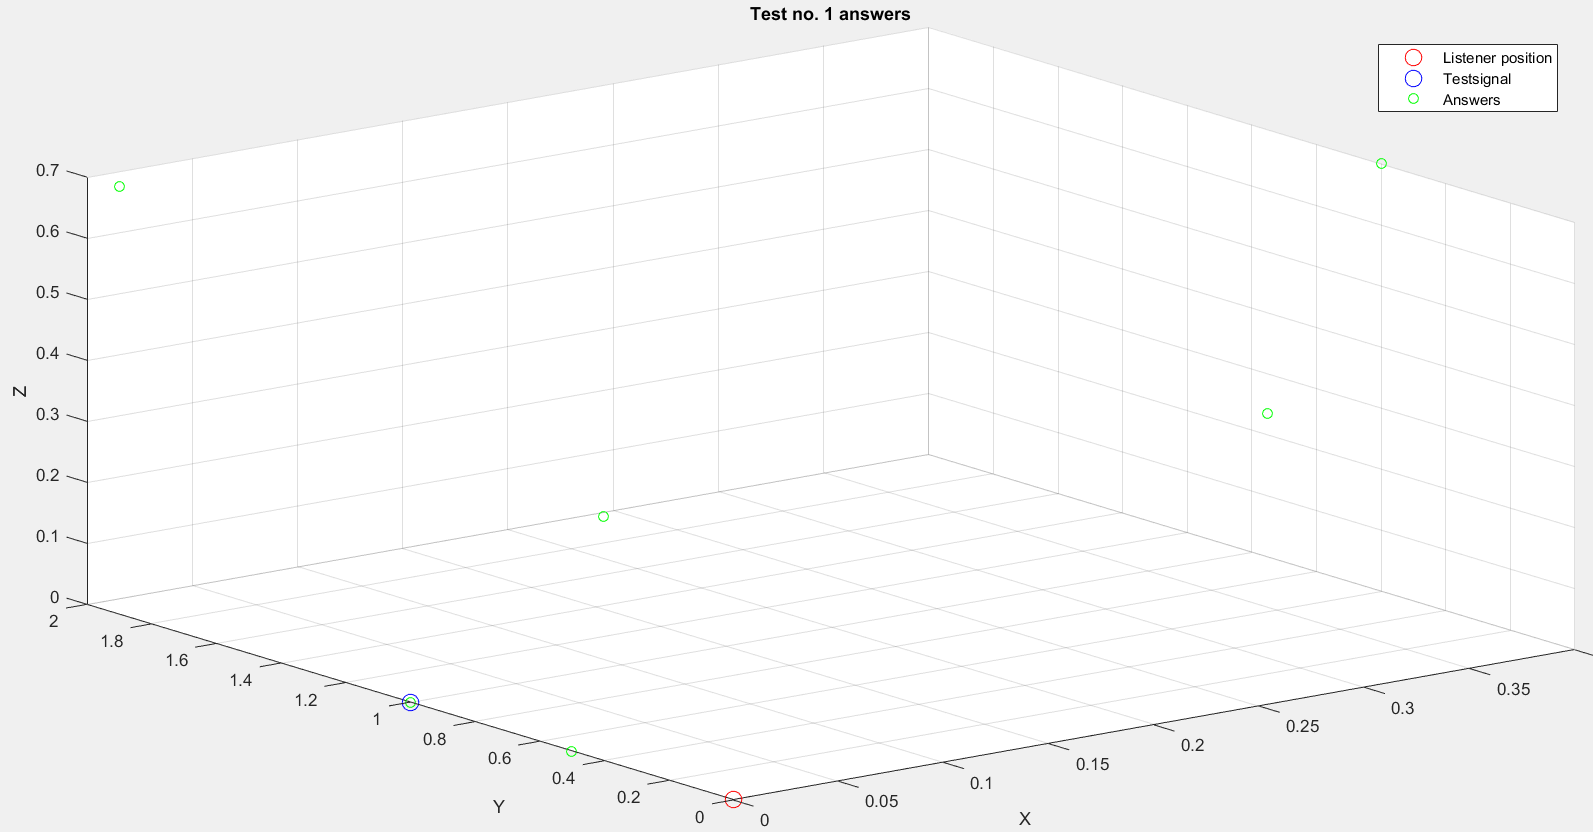
\includegraphics[width=1\linewidth]{All_Pics/test1plot}
	\caption{Plot af svarene for testsignal nr. 1}
	\label{fig:test1plot}
\end{figure}

\begin{figure}[h]
	\centering
	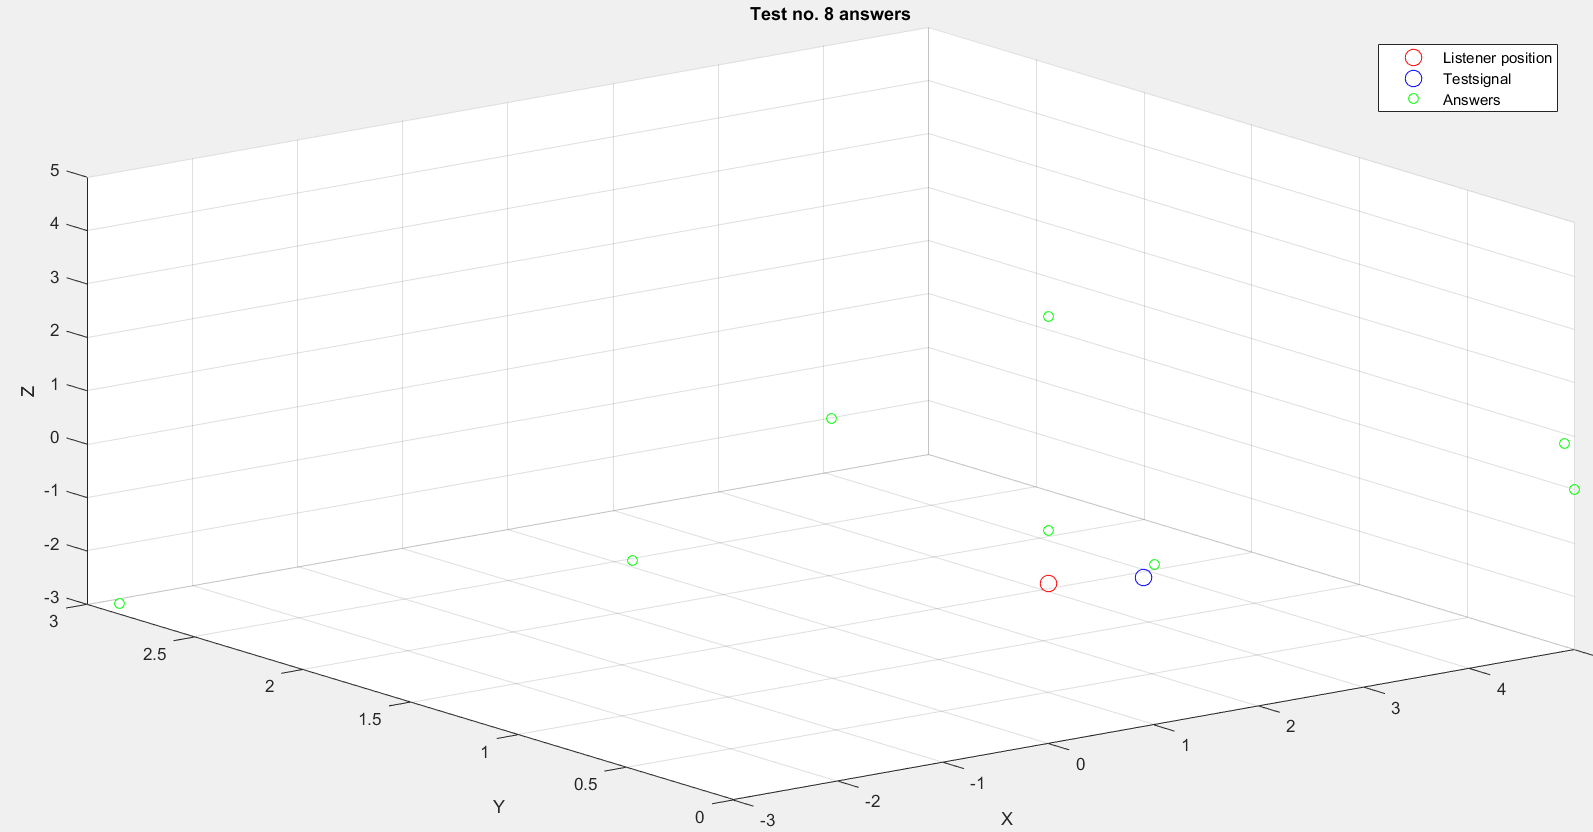
\includegraphics[width=1\linewidth]{All_Pics/test8plot}
	\caption{Plot af svarene for testsignal nr. 8}
	\label{fig:test8plot}
\end{figure}

Dette kan ligeledes konkluderes ud fra figur \ref{fig:test1stat} og figur \ref{fig:test8stat} som viser normalfordelingskurverne ud fra de udregnede middelværdier og standardafvigelser af svarene. Det ses at middelværdierne ligger væsentligt tættere på den aktuelle værdi for testsignal 1, og at kurverne for testsignal 8 er væsentligt bredere, hvilket indikerer en stor spredning i svarene. 

\begin{figure}[h]
	\centering
	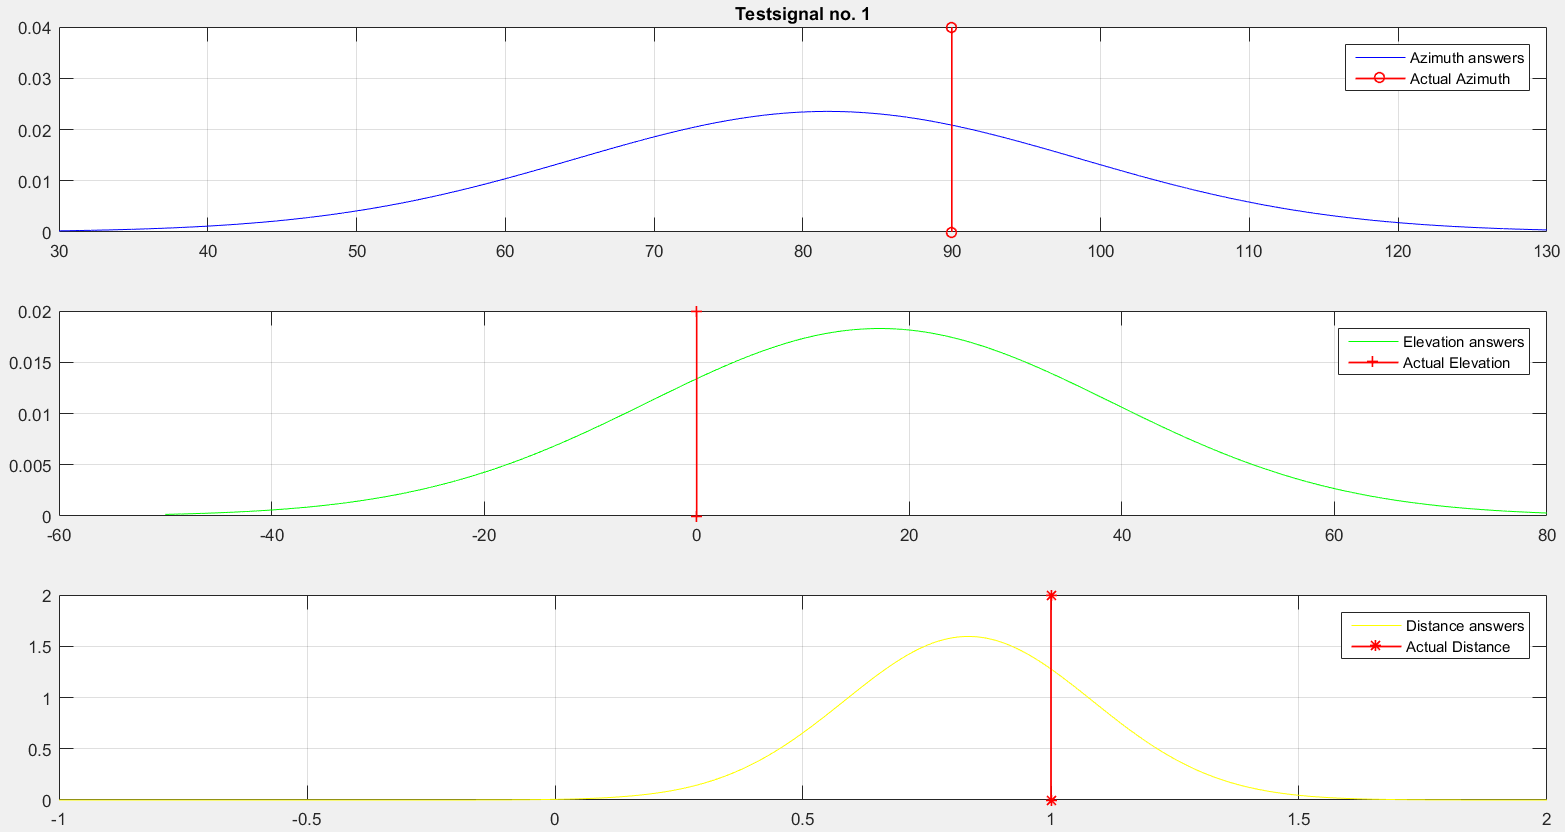
\includegraphics[width=1.1\linewidth]{All_Pics/test1stat}
	\caption{Statistisk normalfordeling af svarene for testsignal nr. 1}
	\label{fig:test1stat}
\end{figure}

\begin{figure}[h]
	\centering
	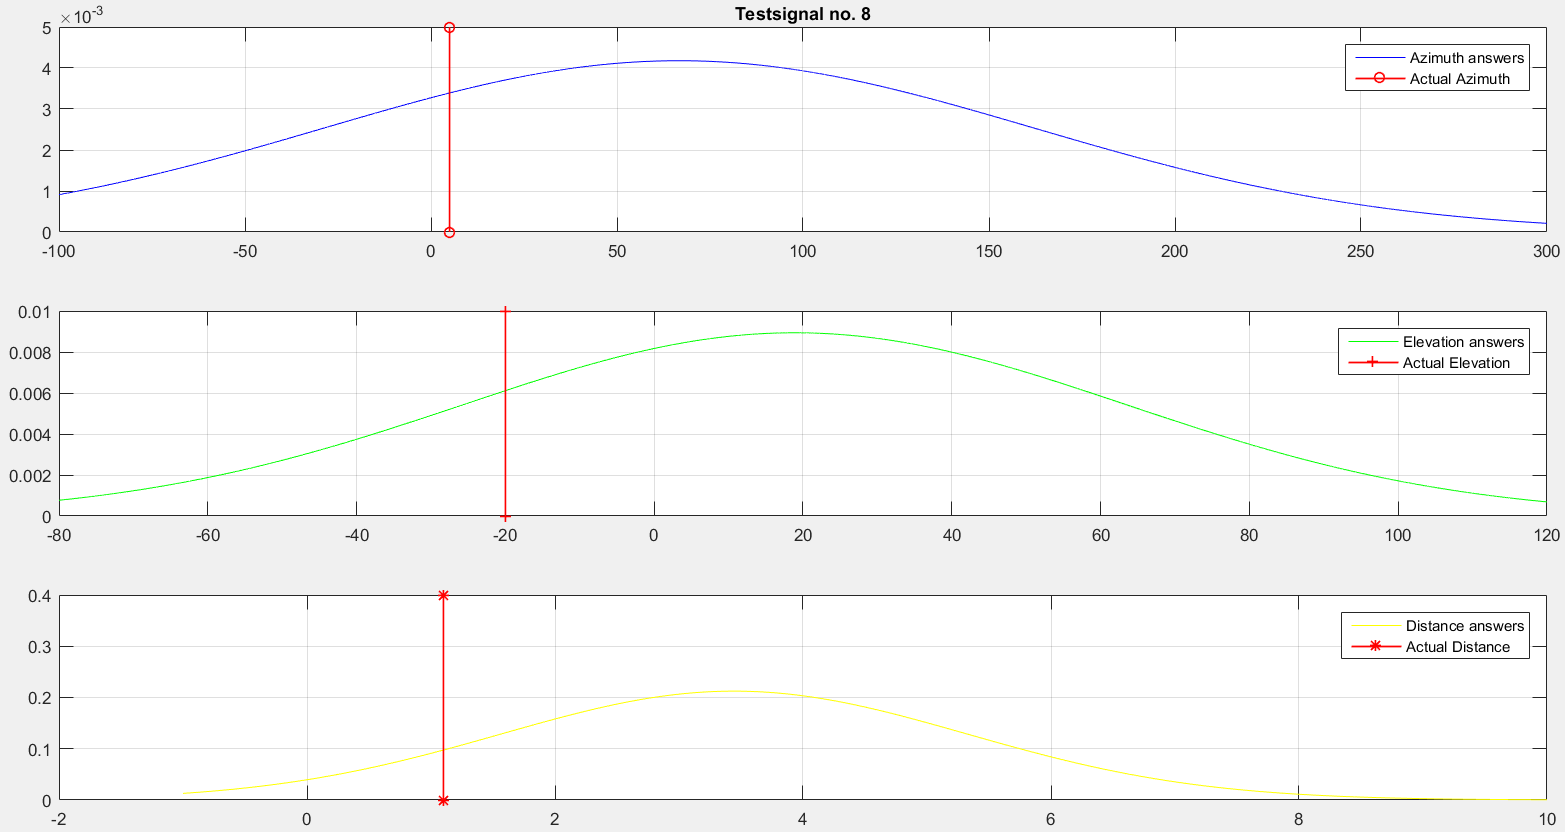
\includegraphics[width=1.1\linewidth]{All_Pics/test8stat}
	\caption{Statistisk normalfordeling af svarene for testsignal nr. 8}
	\label{fig:test8stat}
\end{figure}

Udregner man forskellen mellem de beregnede middelværdier og de aktuelle værdier for både azimuth, elevation og distance, kan man danne sig et overblik over, hvilke testsignaler der har været svære at høre. På figur \ref{fig:resoverblikdiff} kan det ses, at testsignal nr. 9 var det sværeste at høre både når det galt azimuth og elevation, mens det i distancen var signal nr. 6 som var vanskeligst at afgøre. Dette kan bl.a. skyldes, at testsignal nr. 9 var placeret direkte over hovedet af lyttepositionen, som både er en svær position at bedømme i det 'normale' akustiske domæne, samt svært at gengive i det digitale. 
Testsignal nr. 1 er med disse resultater, det signal som er nemmest at bestemme azimuth og distance på, mens det for elevation er signal nr. 10 som var det nemmeste.


\begin{figure}[h]
	\centering
	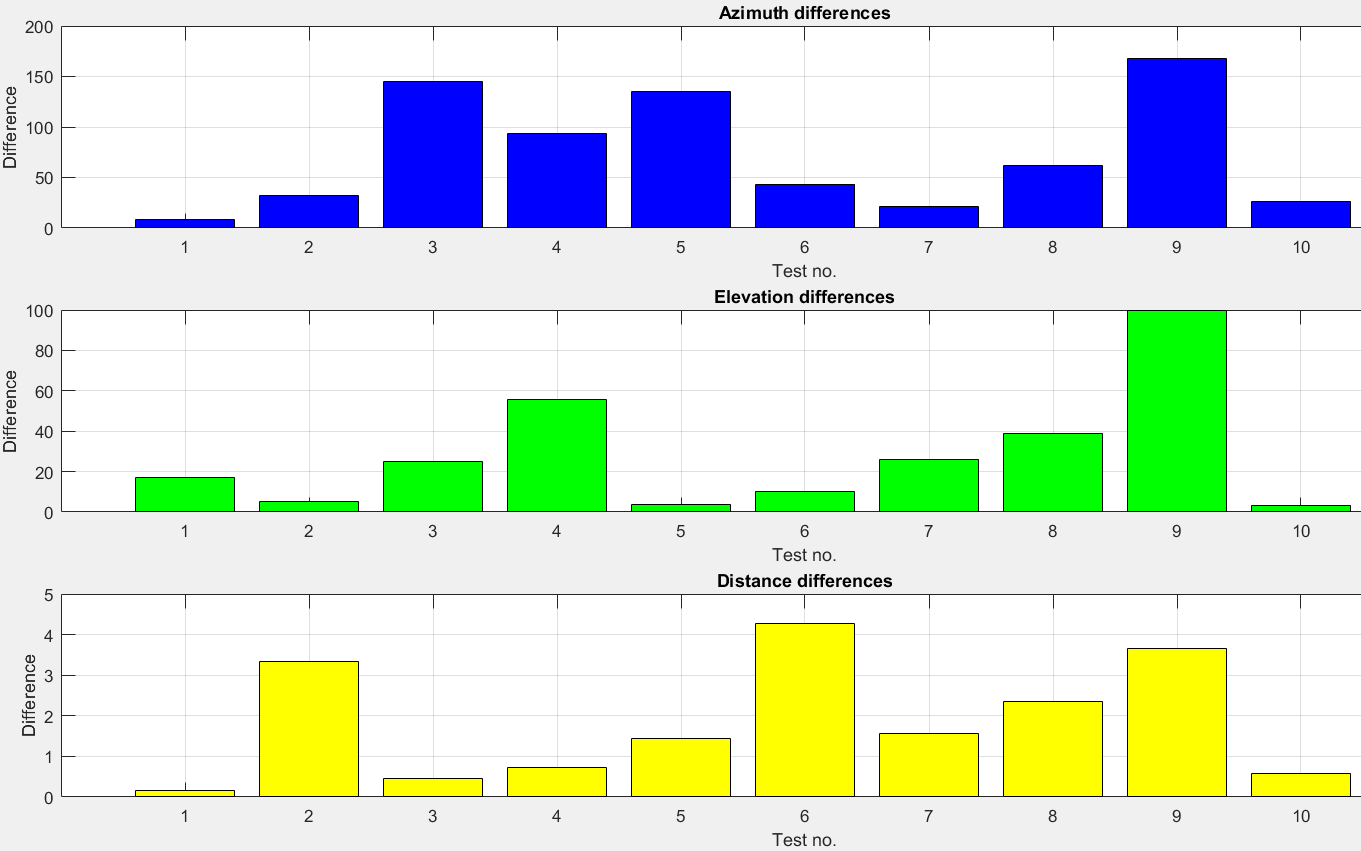
\includegraphics[width=1\linewidth]{All_Pics/resoverblikdiff}
	\caption{Difference udsving mellem den aktuelle position og de midlede testresultater.}
	\label{fig:resoverblikdiff}
\end{figure}






